\section{Problem definition}

In this project, the structure of a parachute is going to be analyzed in order
to obtain the strain and stress of each one of his elements under typical
operation in flight, considering the mass of the system and the drag forces
due to the air.\\

The structure of the parachute to be studied is shown in the figure \ref{fig:definition},
where it's also indicated the types and structure of the materials used for the
bars. This will be of two different types of material, named as "\textit{bars}" and
"\textit{cables}".\\

The parachute consists in a structure of rigid bars and cables which holds a
payload mass of $M = 120kg$, and the system is supposed to descend with constant
low terminal velocity due to the drag produced by the air.

\begin{figure}[h]
	\centering
	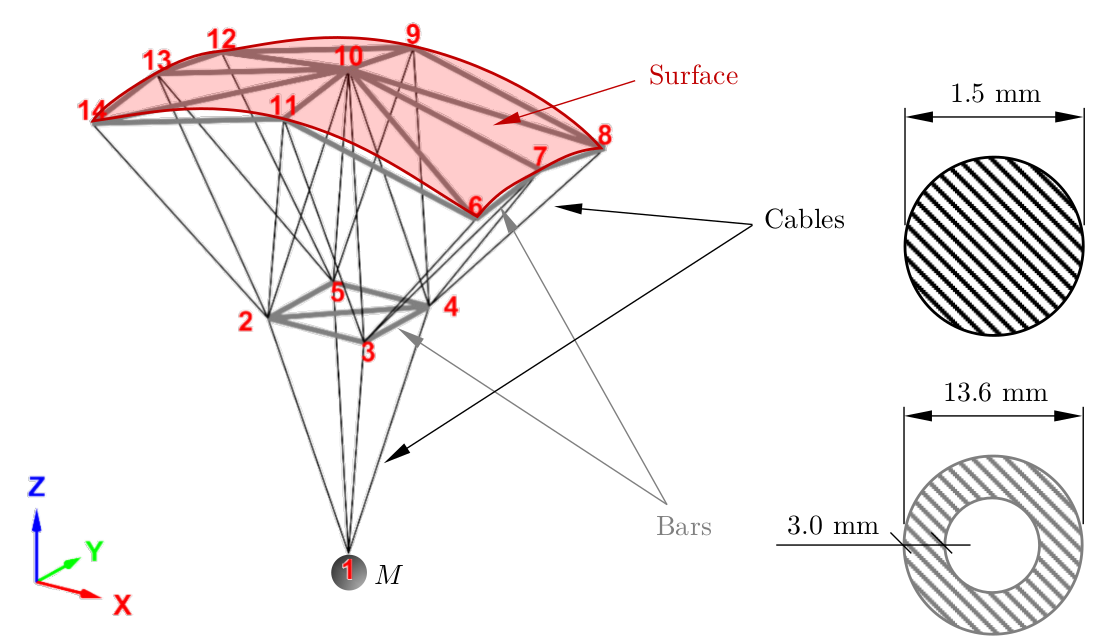
\includegraphics[width=0.8\textwidth]{img/parachute_definition.png}
	\caption{Definition of structure nodes and materials}
	\label{fig:definition}
\end{figure}

Materials properties of \textit{bars} and \textit{cables} are indicated in the
table \ref{tab:materials}.

\begin{table}[h]
\centering
\begin{tabular}{|p{6cm}|c|c|}
\hline
\textbf{Property}  			& \textbf{Cables} & \textbf{Bars} \\ \hline
Density $\rho$ $(kg/m^3)$		& 1500		& 2300	\\ \hline
Young's Modulus E (GPa)			& 200		& 70	\\ \hline
Yield strength $\sigma_{lim}$ (MPa)	& 300		& 240	\\ \hline
Section area A $(mm^2)$			& 1.77		& 57.02	\\ \hline
\end{tabular}
\caption{Materials definition}
\label{tab:materials}
\end{table}

The upper surface is made with a fabric with the following properties:

\begin{itemize}
	\item Density $\rho_S = 1500 kg/m^3$
	\item Surface area $S = 17.5m^2$
	\item Thickness $t_S = 1mm$
	\item Drag coefficient $C_D = 1.25$
\end{itemize}

Considering the air density to be $\rho_{air} = 1.225$ $kg/m^3$ and the gravity
acceleration $g_0 = 9.81$ $m/s^2$

\subsection{Input data}

In order to sole the problem, some input data has been taken into account.
Firstly we define a matrix with the coordinates of the nodes. This first matrix's
dimension is 14x3, where the row index represents the node number, and the three columns
are the cartesian coordinates in meters.

\begin{table}[h]
\centering
\begin{tabular}{|c|c|c|c|}
\hline
\textbf{Node number} & \textbf{x(m)} & \textbf{y(m)} & \textbf{z(m)} \\ \hline
1 & 	0.000 	&	 0.000  	& 0.000	\\ \hline
2 & 	-0.725	&	 -0.731  	& 3.250	\\ \hline
3 & 	0.725 	&	-0.731  	& 3.250	\\ \hline
4 & 	0.725 	&	 0.731  	& 3.250	\\ \hline
5 & 	-0.725	&	  0.731  	& 3.250	\\ \hline
6 & 	2.900 	&	-1.450  	& 5.630	\\ \hline
7 & 	2.900 	&	 0.000  	& 5.820	\\ \hline
8 & 	2.900 	&	 1.450  	& 5.630	\\ \hline
9 & 	0.000 	&	 1.450  	& 6.340	\\ \hline
10 & 	0.000 	&	 0.000  	& 6.530	\\ \hline
11 & 	0.000 	&	-1.450  	& 6.340	\\ \hline
12 & 	-2.900	&	  1.450  	& 5.630	\\ \hline
13 & 	-2.900	&	  0.000  	& 5.820	\\ \hline
14 & 	-2.900	&	 -1.450  	& 5.630	\\ \hline
\end{tabular}
\caption{Node coordinates}
\label{tab:coordinates}
\end{table}

\newpage
\section{Results}

After running the code the following results are obtained.\\

\subsection{Strain \& Stress}

The tables \ref{tab:strain} \& \ref{tab:stress} shows the values of strain and stress obtained for each element
(bar or cable).

\begin{table}[h]
\centering
\begin{tabular}{|c|c|c|c|}
\hline
\textbf{Element number} & \textbf{Strain} ($10^{-5}$) & \textbf{Element number} & \textbf{Strain} ($10^{-5}$) \\ \hline
1 &   87.30 &  22 &  21.76 \\ \hline
2 &   87.41 &  23 &  18.63 \\ \hline
3 &   87.30 &  24 &  41.27 \\ \hline
4 &   87.41 &  25 &  21.10 \\ \hline
5 &    1.16 &  26 &  -0.94 \\ \hline
6 &   -1.18 &  27 &  -0.86 \\ \hline
7 &    1.16 &  28 &  -1.72 \\ \hline
8 &   -1.18 &  29 &  -0.05 \\ \hline
9 &    0.00 &  30 &  -2.43 \\ \hline
10 &   18.74 &  31 &  -0.05 \\ \hline
11 &   21.88 &  32 &  -1.72 \\ \hline
12 &   21.16 &  33 &  -0.94 \\ \hline
13 &   41.27 &  34 &  -0.86 \\ \hline
14 &   41.27 &  35 &  -0.94 \\ \hline
15 &   21.10 &  36 &  -0.05 \\ \hline
16 &   18.63 &  37 &  -2.43 \\ \hline
17 &   21.76 &  38 &  -1.72 \\ \hline
18 &   21.16 &  39 &  -0.94 \\ \hline
19 &   41.27 &  40 &  -0.05 \\ \hline
20 &   21.88 &  41 &  -1.72 \\ \hline
21 &   18.74 &   &   \\ \hline
\end{tabular}
\caption{Strain per element}
\label{tab:strain}
\end{table}

\begin{table}[h]
\centering
\begin{tabular}{|c|c|c|c|}
\hline
\textbf{Element number} & \textbf{Stress (MPa)} & \textbf{Element number} & \textbf{Stress (MPa)} \\ \hline
1 &  174.61  &  22 &  43.53305 \\ \hline
2 &  174.82  &  23 &  37.26479 \\ \hline
3 &  174.61  &  24 &  82.55799 \\ \hline
4 &  174.82  &  25 &  42.19999 \\ \hline
5 &    0.81  &  26 &  -0.66369 \\ \hline
6 &   -0.82  &  27 &  -0.60296 \\ \hline
7 &    0.81  &  28 &  -1.20673 \\ \hline
8 &   -0.82  &  29 &  -0.03722 \\ \hline
9 &    0.00  &  30 &  -1.70267 \\ \hline
1 &    37.49 &   31 &  -0.03636 \\ \hline
1 &    43.77 &   32 &  -1.20870 \\ \hline
1 &    42.32 &   33 &  -0.66194 \\ \hline
1 &    82.55 &   34 &  -0.60296 \\ \hline
1 &    82.55 &   35 &  -0.66369 \\ \hline
1 &    42.19 &   36 &  -0.03722 \\ \hline
1 &    37.26 &   37 &  -1.70267 \\ \hline
1 &    43.53 &   38 &  -1.20673 \\ \hline
1 &    42.32 &   39 &  -0.66194 \\ \hline
1 &    82.55 &   40 &  -0.03636 \\ \hline
2 &    43.77 &   41 &  -1.20870 \\ \hline
2 &    37.49 &    &   \\ \hline
\end{tabular}
\caption{Stress per element}
\label{tab:stress}
\end{table}

The \textbf{total mass} of the structure is calculated summing the mass of the payload,
the parachute upper surface and the mass of every bar or cable, which are
calculated taking into account the material density, length and cross section
area. Doing this, the total mass is:

\begin{equation}
	\boxed{M_{tot} = 152.73 kg}
\end{equation}

The \textbf{terminal velocity} of the parachute is calculated by assuming that, in this
steady state, the summation of vertical forces will be zero, i.e., the drag
created by the upper surface will equal the total weight of the parachute. Given
that the drag is:

\begin{equation}
	M_{tot} g_0 = W = D = \frac{1}{2}C_D S \rho_{air} V_t^2
\end{equation}

We can obtain the terminal velocity as:

\begin{equation}
	\boxed{V_t = \sqrt{\frac{2W}{S C_d\rho_{air}}} = 10.575 ~ m s^{-1}}
\end{equation}

We can also compute the \textbf{safety factor under normal operating conditions}. This
consists in compare the actual stress suffered by the materials (bars and cables),
with the yield strength of each material. This is an important factor because, if
we overtake it, some of the materials could enter in his plastic deformation region,
producing perpetual deformations or even material failures.\\

This factor is calculated in the following way:
\begin{equation}
	SF = min\left(\frac{\sigma_{lim}}{|\sigma|}\right)
\end{equation}

, where $\sigma_{lim}$ is the yield strength, and $\sigma$ is the actual stress
suffered by the element. The smaller, closer to 1, this factor, the most risk of
failure.

Finally, the safety factor is found in the the cable number 4, with a value of:
\begin{equation}
	\boxed{SF = 1.716}
\end{equation}

The \textbf{risk of buckling} can also be computed using the next expression:

\begin{equation}
	\sigma_{cr} = \frac{E \pi^2}{(L/r)^2}
\end{equation}

, where r, in the case of a circular shaft is $a/2$, $a$ the radius of the shaft.

Computing this just for bars under compression, we obtain that the worst safety factor
for buckling is observed in the bar 37 with a value of

\begin{equation}
	\boxed{SF_{buckling} = 2.5\cdot10^8}
\end{equation}

\newpage
\subsection{Plots of the deformed structure}

\begin{figure}[h]
	\centering
	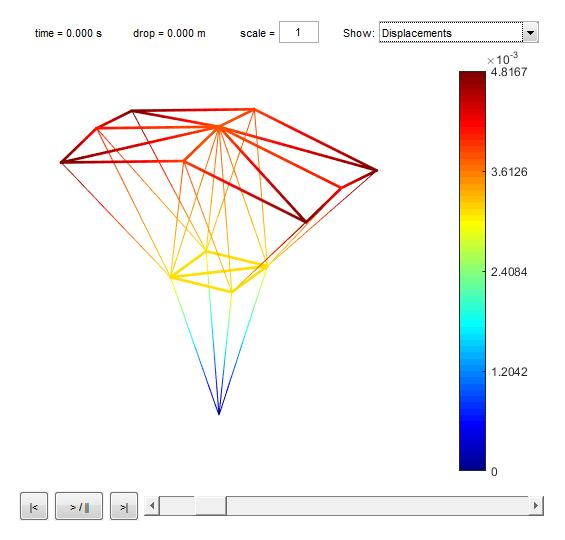
\includegraphics[width=0.8\textwidth]{img/displacements1.jpg}
	\caption{Displacements under normal conditions}
	\label{fig:displacements}
\end{figure}

\begin{figure}[h]
	\centering
	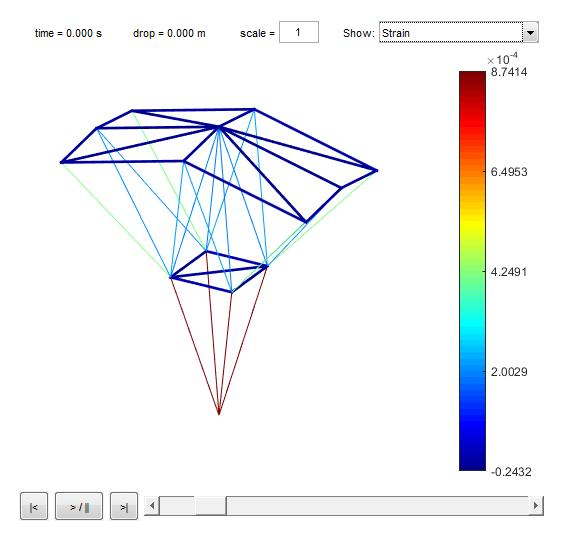
\includegraphics[width=0.8\textwidth]{img/strain1.jpg}
	\caption{Strains under normal conditions}
	\label{fig:strain}
\end{figure}

\begin{figure}[h]
	\centering
	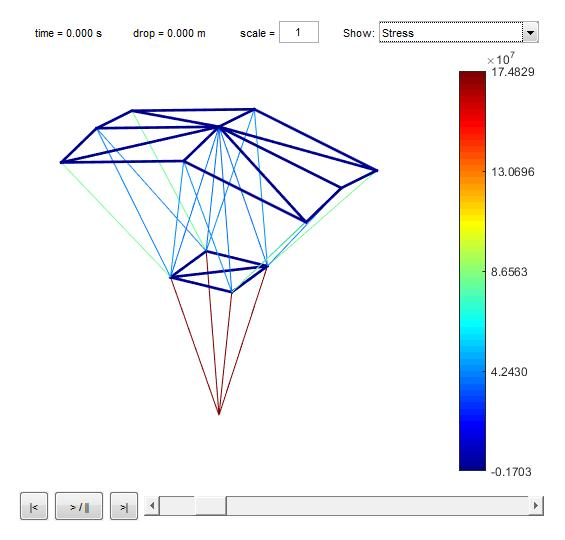
\includegraphics[width=0.8\textwidth]{img/stress1.jpg}
	\caption{Stress under normal conditions}
	\label{fig:stress}
\end{figure}
